%===============================================================================
% Bayesian Variable-order Markov Models
% Kevin Durant
% March 2019
%===============================================================================

\documentclass[12pt,a4paper]{article}

\usepackage[hscale=0.666667,vscale=0.747547]{geometry}
\usepackage{microtype}
\usepackage{mathtools} % also loads amsmath.
\usepackage{iftex}
\ifPDFTeX
  \usepackage[T1]{fontenc}
  \usepackage[utf8]{inputenc}
  \usepackage{amssymb}
\else
  % Load after other font- or maths-related packages (loads amsmath and fontspec
  % if necessary). Sets a custom version of Latin Modern Math by default.
  \usepackage{unicode-math}
  % \setmainfont{XITS}
  % \setmathfont{XITS Math}
\fi
\usepackage{booktabs} % better-looking tables.
\usepackage{pgfplots}
\usepackage{hyperref}

% Package settings %============================================================

\usepgfplotslibrary{fillbetween,statistics}
\pgfplotsset{compat=1.16,width=0.75\textwidth}
\pgfplotsset{every axis plot/.append style={very thick}}
\definecolor{cbblue}{RGB}{31,119,180}
\definecolor{cborange}{RGB}{255,127,14}

% Custom maths commands %=======================================================

\newcommand\ds{\displaystyle}                 % large maths.
\newcommand\ts{\textstyle}                    % small maths.
\newcommand\mb[1]{\mathbb{#1}}                % mathbb shorthand.
\newcommand\mc[1]{\mathcal{#1}}               % mathcal shorthand.
\newcommand\ub[1]{\symbf{#1}}                 % unicode-math symbf shorthand.
\newcommand\ff[1]{^{\underline{#1}}}          % falling factorial.
\newcommand\rf[1]{^{\overline{#1}}}           % rising factorial.
\newcommand\ul[1]{\underline{#1}}             % underline.
\newcommand\ol[1]{\overline{#1}}              % overline.
\DeclareMathOperator\Pb{P}                    % probability.
\DeclareMathOperator\Ex{E}                    % expected value.
\DeclareMathOperator\Va{V}                    % variance.
\DeclarePairedDelimiter\lr{\lparen}{\rparen}  % sized parentheses.
\DeclarePairedDelimiter\lrb{\lbrack}{\rbrack} % sized brackets.
\DeclarePairedDelimiter\abs{\lvert}{\rvert}   % absolute value symbol.
\DeclarePairedDelimiter\cl{\lceil}{\rceil}    % ceiling symbol.
\DeclarePairedDelimiter\fl{\lfloor}{\rfloor}  % floor symbol.

% Document-specific maths commands %============================================

\newcommand\peq{\mathop{=}}   % tight equals (used in probabilities).
\DeclareMathOperator\cat{Cat} % categorical distribution.
\DeclareMathOperator\dir{Dir} % Dirichlet distribution.
\DeclareMathOperator*{\argmax}{arg\,max}

% Title %=======================================================================

\title{Bayesian Variable-order Markov Models}
\author{Kevin Durant}
\date{}

% Document %====================================================================

\begin{document}

\maketitle

\begin{abstract}
To do:
\begin{itemize}
  \item Use `symbol' and `character' consistently.
\end{itemize}
\end{abstract}

\section{Introduction} %========================================================

% A year or two ago, while working on a problem involving temporal communication
% networks (in which the underlying edge events are all timestamped, and thus
% ordered), a peripheral question arose that seemed worth trying to answer:
% \textit{are there any directed paths within the network that are particularly
% predictable?} Phrased another way: \textit{are there nodes in the network whose
% outgoing edges can be predicted based on their most recent incoming edges? And
% to what depth?}

% Dependencies such as these are interesting in the context of communication
% networks because they point to the presence of certain message-passing `chains'.
% For example, it might be the case that whenever a node~$B$'s most recent
% incoming message originated at node~$A$, the next message sent by~$B$ is likely
% to be to some third node~$C$. If this is not the usual behaviour for messages
% sent from~$B$, then the distribution of its outgoing edges is conditionally
% dependent on its last incoming edge. We are interested in determing, for a given
% network, to what extent---if any---this dependence holds. And specifically: with
% respect to which nodes, which incoming edges, and to what depth.

% The problem can also be stated without the need for network terminology, for
% with a bit of thought one sees (Section~\ref{sec:templ soc netw}) that each
% uninterrupted path within a temporal network can also be represented as a
% sequence of nodes, and thus simply as a string of symbols~$x_1 x_2 \dots x_N$.
% The objective then is to find substrings~$x_{n-k} \dots x_{n-1}$ that allow the
% next symbol~$x_n$ to be predicted (to some extent), for we can then
% regard~$x_{n-1}$ as conditionally dependent on the depth~$k-1$ substring for the
% purpose of predicting the symbol~$x_n$ that follows it.

% It is perhaps worth mentioning here that we are not interested in dependence on
% any sort of transformed substring

% The obvious probabilistic framework to adopt when approaching this problem is
% that of Markov chains, however it's worth emphasising the fact that our interest
% is not so much in modelling the outgoing edge distribution of each node to some
% depth for the purposes of prediction, but rather in pruning the set of all
% Markov states until only those that are truly useful for prediction of their
% next edge remain.

% on a per-case basis, whether the Markov assumption is a reasonable one; and to
% what order in each case. Since independence from any directly preceding symbols
% can be viewed as a Markov property of order zero, we can find significant
% subsequences by assuming the Markov property throughout, and asking what order
% is most likely in each case.





% It would be interesting (in our humble opinion) to
% know edge to terminate at~$B$ node~$B$'s incoming edges is~$A \longrightarrow
% B$, and the next edge involving~$B$ is~$B \longrightarrow C$, then 

% With regard to the second phrasing of the question above, it's worth emphasising
% the use of the phrase `certain the fact that we are not trying to answer the question of whether a given node's
% incoming edges are significant \emph{in general}, but rather \emph{which} of its
% incoming neighbours (if any) are useful for prediction, in what way, and to what
% depth.


% \textit{are certain directed paths
% within the network more predictable than others?} Or, phrased another way:
% \textit{are there sequences of edges that reliably determine the edges that
% follow them?} In essence, we were curious to know whether there were elements of
% the data that could be said to be strongly influenced by those that directly
% preceded them; and if so, to determine these elements algorithmically.

% Of course the social networks that sparked the search for repetitive were simply
% a particular (and convenient) way of viewing a set of sequential data---any
% sequence of symbols from a given alphabet can be viewed in the same way. So the
% above question should really be phrased with respect to arbitrary sequences
% instead: assuming that the Markov property holds for 

\section{Methodology} %=========================================================

Let \(\ub{x} = x_1, x_2, \dotsc\) be a sequence of random variables. For the
purpose of inference we assume that the process that generates \(\ub{x}\) is
Markovian, and that the state that any symbol~\(x_n\) depends on is some
function of the preceding values~\(x_1, \dots, x_{n-1} = \ub{x}_{1:n-1}\). Every
state implies a discrete probability distribution over the symbol
alphabet~\(\mc{A}\), and it is according to these distributions that the
sequence is generated.

% If \(x_n\) is generated by some process that does not depend on these values,
% then the distribution of \(x_n\) conditioned on any subset of \(x_1, \dots,
% x_{n-1}\) will simply be equal to its marginal distribution~\(\Pb(x_n)\).

A \emph{set} of states~\(\mc{S}\) defines a Markov model that can be used to fit
the data, and to some extent the states of such a model are a description, or
assumption, of the dependence and independence relationships among the random
variables. In the trivial case \(\mc{S} = \{\lambda\}\), every symbol is
generated from the same state according to some common distribution, and thus
every symbol~\(x_n\) is independent of its predecessors: 
\begin{align*}
  \Pb\lr{x_n, \ub{x}_{1:n-1} \mid \mc{S}} &=
    \Pb\lr{x_n \mid \ub{x}_{1:n-1}, \mc{S}}
    \Pb\lr{\ub{x}_{1:n-1} \mid \mc{S}} \\
  &= \Pb\lr{x_n \mid \mc{S}} \Pb\lr{\ub{x}_{1:n-1}, \mc{S}}.
\end{align*}
Note however that \(x_n\) is only \emph{conditionally} independent of the other
symbols in light of the model \(\mc{S}\), and that different models suggest
different dependencies. For example let \(\mc{S} = \{\lambda, a\}\), and assume
that the state of a subsequence~\(x_{1:n-1}\) is \(a\) if \(x_{n-1} = a\) and
\(\lambda\) otherwise. In this case \(x_n\) is not necessarily independent of
\(x_{n-1}\), since
\begin{equation*}
  \Pb\lr{x_n, x_{n-1} \peq a \mid \mc{S}} =
    \Pb\lr{x_n \mid x_{n-1} \peq a, \mc{S}} \Pb\lr{x_{n-1} \peq a \mid \mc{S}},
\end{equation*}
and \({\Pb(x_n \mid x_{n-1} \peq a, \mc{S})}\) is not in general equal to
\(\Pb(x_n \mid \mc{S})\) for all possible values of \(x_n\).

The idea here is to define a set of models~\(\mc{M}\) that covers as many of the
dependence/independence relationships among the sequence's random variables as
possible. Assuming one has access to the marginal likelihood (also called the
\emph{evidence}) corresponding to each model, one can perform model comparison
to get an idea of which variables are likely independent of one another given
the space of potential models.

Possibly the most interesting question to ask in this type of scenario is `What
is the probability that \(x_n\) is independent of \(x_{n-1}\) given \(\mc{M}\)?'
A second, related question is `What is the probability that state \({x_{n-1} =
a}\) is present in the underlying model~\(\mc{S}^*\)? We will focus on the
latter question for now, since it follows directly from the posterior
distribution over the space of models. Unfortunately though, this distribution
is computationally intractable due to the numer of potential dependencies among
the random variables. One way of dealing with intractable distributions---even
discrete ones such as this---is to draw samples according to the unnormalised
posterior function by means of a Markov chain Monte Carlo algorithm.

Even with this approach, however, one needs to specify states on the symbol
level to make the modelling tractable, and limit the number of possible models
in some way so that MCMC can be performed. A simple variable-order Markov model
approach to the modelling problem satisfies both of these constraings, and the
limitations it imposes seem sensible enough that it may still prove useful when
applied to relatively simple problems (such as those we are interested in here).
The states we restrict ourselves to here are those that result from permuting
the subsequence \(\ub{x}_{1:n-1}\) and then truncating all but its last \(k\)
symbols:~\(f(\ub{x}_{1:n-1}) = x_{\phi(n-k)}, \dots, x_{\phi(n-1)}\). In the
simplest case---the identity permutation---states are nothing but prefixes of
length \(k\) (although we will use the term `prefix' regardless of the
permutation function~\(\phi\)).

Any set of prefixes of this form can be arranged in a tree in which they appear
as leaves: by letting the root node represent the empty prefix (a valid state),
its children the single-symbol states~\({\{\,x_{n-1} = a : a \in \mc{A}\,\}}\),
and so on. A complete tree of depth \(k\) then corresponds to a \(k\)th-order
Markov model. By considering incomplete trees as well, however, we obtain
\emph{variable}-order Markov models, in which the state
function~\(f(\ub{x}_{1:n-1})\) is able to yield prefixes of arbitrary length
according to the root-leaf paths in the tree.

To avoid the situation in which a subsequence~\(\ub{x}_{1:n-1}\) cannot be
mapped to a leaf node of the state tree (this can occur when considering the
first few variables in the sequence, whose prefixes are very short), we consider
every node in the tree to be a valid state. An alternative strategy would be to
invent symbols so as to extend the prefix to a leaf node, as is done by
Rissanen.

Our final set of models~\(\mc{M}\) is thus the set of all possible \(M\)-ary
trees, which need be neither full nor complete. As mentioned above, every such
model~\(\mc{S} \in \mc{M}\) suggests a dependence structure for the random
variables in the sequence; the actual details of the dependencies, however, are
given by unknown conditional distributions~\(\Pb(x_n \mid \ub{x}_{1:n-1} = s)\)
for each state~\(s \in \mc{S}\).

For the purposes of prediction, compression, or parameter estimation, one would
usually select one specific model~\(\mc{S}\)---believed to be sufficient for
capturing all of the dependencies that may be present in the data---and then
attempt to infer the conditional distributions~\(\Pb(x_n \mid s)\) in some way,
perhaps taking measures to avoid overfitting.

Assuming that this problem can be solved to some reasonable degree---yielding a
maximum likelihood solution, or a posterior distribution over the space of
possible sets of distributions, or a representative sample from this
posterior---one can then proceed a step further, and begin to compare the
appropriateness of different models from the set~\(\mc{M}\). The reason for
doing so might be to perform model selection or model averaging to improve the
accuracy of prediction, or---and this is our goal here---one may simply want to
compare models for the sake of better understanding the underlying process that
generated the data. In our specific case, we hope to have constructed our set of
models in such a way that their relative likelihoods will allow us to infer
which sequences of symbols have a significant effect on their immediate
successors.

The form of Markov model we have described here is intended to be minimal, in
the sense that it encodes the effect of a symbol's prefix and nothing more. If a
symbol~\(x_n\) is generated by some other mechanism that is in fact independent
of the prefix~\(x_{\phi(n-k)}, \dots, x_{\phi(n-1)}\), then models that include
this state should lead to lower marginal likelihoods than those that do not.

Conversely, if we find that this node appears regularly among the state trees
(relative to the posterior distribition over \(\mc{M}\)) we may conclude that
the occurrence of the prefix in the data can to some extent be used to predict
the symbols that will follow. This Markovian dependence may take different
forms: it might be that \(x_n\) depends solely on a symbol \(m\) steps
prior,~\(x_{n-m}\), or it may be that the entire prefix has an influence. These
dependencies can all be desribed within the state tree framework---albeit some
more naturally and easily than others.

Following on from the discussion above, there are two problems that must be
solved: we must infer the conditional distributions~\(\{\,\Pb(x_n \mid s) : s
\in \mc{S}\,\}\), and then use this information to compare the relative
(marginal) likelihoods of the models~\(\mc{M}\).

\subsection{Bayesian variable-order Markov models} %============================

Let \(\mc{S} \in \mc{M}\) be one of the variable-order Markov models described
above, and for each of its states~\(s\) let \(\ub{n}_s\) be a vector containing,
for each symbol~\(x \in \mc{A}\), the number of times that the prefix
corresponding to \(s\) is followed by \(x\) when it occurs in the data. We
choose to model the data-generating process using a categorical distribution for
each state:
\begin{equation*}
  \Pb\lr{x \mid s} = \cat\lr{\ub{p}_s},
\end{equation*}
where \(\ub{p}_s\) is another vector of length \(L = \abs{\mc{A}}\)---in this
case one of symbol probabilities. The first object of inference is the set of
vectors~\(\ub{\theta} = \{\,\ub{p}_s : s \in \mc{S}\,\}\), which we can estimate
in a fully Bayesian manner. The likelihood of a given set of
parameters~\(\ub{\theta}\) is:
\begin{align*}
  \Pb\lr{\ub{x}_{1:n} \mid \ub{\theta}, \mc{S}} &= \Pb\lr{x_1 \mid \lambda}
    \Pb\lr{x_2 \mid f_{\mc{S}}\lr{x_1}} \dotsm
    \Pb\lr{x_n \mid f_{\mc{S}}\lr{\ub{x}_{1:n-1}}} \\
  &= \prod_i \Pb\lr{x_i \mid f_{\mc{S}}\lr{\ub{x}_{1:i-1}}},
\end{align*}
where once again \(f_{\mc{S}}(\ub{x})\) maps sequences to states, and empty
sequences map to the null state \(\lambda\).

A conjugate prior of the categorical distribution is the Dirichlet distribution,
so for each state's unknown probability vector~\(\ub{p}_s\) we assume:
\begin{equation*}
  \Pb\lr{\ub{p}_s} = \dir\lr{\ub{\alpha}}.
\end{equation*}
Here \(\ub{\alpha}\) is a vector of \(L\) `concentration' parameters, which can
be thought of as symbol occurrences that have been counted prior to observing
the data. In practice a symmetric Dirichlet ditribution will often be used,
e.g.~\(\ub{\alpha} = \ub{1}\).

The posterior that arises when a categorical likelihood function is paired with
a Dirichlet prior is itself a Dirichlet distribution---one in which the
concentration parameter consists of occurrence counts. In our case, multiple
categorical distributions are involved, each with its own prior (although we
assume that these priors are identical). Due to the mutual independence of each
state's probability vector, however, the situation is no more complicated than
that of a single categorical distribution:
\begin{align*}
  \Pb\lr{\ub{\theta} \mid \ub{x}, \mc{S}} &=
    \frac{\Pb\lr{\ub{x} \mid \ub{\theta}, \mc{S}}
    \Pb\lr{\ub{\theta} \mid \mc{S}}}
    {\int \Pb\lr{\ub{x}, \ub{\theta} \mid \mc{S}}\, d\theta} \\
  &= \frac{1}{Z} \prod_i \Pb\lr{x_i \mid f_{\mc{S}}\lr{\ub{x}_{1:i-1}}}
    \prod_s \Pb\lr{\ub{p}_s} \\
  &= \frac{1}{Z} \prod_s \prod_x \ub{p}_s(x)^{\ub{n}_s(x)} \prod_s
    \frac{1}{\Beta\lr{\ub{\alpha}}} \prod_x \ub{p}_s(x)^{\ub{\alpha}(x)-1} \\
  &= \frac{1}{Z} \prod_s \frac{1}{\Beta\lr{\ub{\alpha}}}
    \prod_x \ub{p}_s(x)^{\ub{n}_s(x)+\ub{\alpha}(x)-1}.
\end{align*}
We have used function notation here to denote the element of a vector
corresponding to a given symbol, for example \(\ub{p}_s(x)\) is the
(categorical) probability of \(x\) given state~\(s\).

Note that the probability vectors~\(\ub{p}_s\) appear separately in the above
posterior probability density function, since we have implicitly assumed that
they are conditionally independent given \(\ub{x}\):
\begin{equation*}
  \Pb\lr{\ub{\theta} \mid \ub{x}, \mc{S}} =
    \prod_s \Pb\lr{\ub{p}_s \mid \ub{x}, \mc{S}}.
\end{equation*}
Each of these independent posteriors is also a Dirichlet distribution, as
expected:
\begin{align*}
  \Pb\lr{\ub{\theta} \mid \ub{x}, \mc{S}} &=
    \frac{1}{Z} \prod_s \frac{1}{\Beta\lr{\ub{\alpha}}}
    \prod_x \ub{p}_s(x)^{\ub{n}_s(x)+\ub{\alpha}(x)-1} \\
  &= \frac{1}{Z} \prod_s \frac{\Beta\lr{\ub{n_s} + \ub{\alpha}}}
    {\Beta\lr{\ub{\alpha}}} \frac{1}{\Beta\lr{\ub{n_s} + \ub{\alpha}}}
    \prod_x \ub{p}_s(x)^{\ub{n}_s(x)+\ub{\alpha}(x)-1} \\
  &= \frac{1}{Z} \prod_s \frac{\Beta\lr{\ub{n_s} + \ub{\alpha}}}
    {\Beta\lr{\ub{\alpha}}} \dir\lr{\ub{n}_s + \ub{\alpha}} \\
  &= \prod_s \Pb\lr{\ub{p}_s \mid \ub{x}, \mc{S}}.
\end{align*}

Since the integral of \(\Pb(\ub{\theta} \mid \ub{x}, \mc{S})\) with respect to
the set~\(\{\,\ub{p}_s\,\}\) is \(1\), we also have:
\begin{align*}
  \Pb\lr{\ub{x} \mid \mc{S}} =
  \int \Pb\lr{\ub{x}, \ub{\theta} \mid \mc{S}}\, d\ub{\theta}
  &= \prod_s \frac{\Beta\lr{\ub{n}_s + \ub{\alpha}}}{\Beta\lr{\ub{\alpha}}} \\
  &= \prod_s \frac{\Gamma\lr*{\sum_x \ub{\alpha}(x)}}
    {\Gamma\lr*{N + \sum_x \ub{\alpha}(x)}} \prod_x
    \frac{\Gamma\lr{\ub{n}_s(x) + \ub{\alpha}(x)}}{\Gamma\lr{\ub{\alpha}(x)}},
\end{align*}
where \(N = \sum_x \ub{n}_s(x)\). This value---the marginal likelihood of the
model~\(\mc{S}\)---is what we are most interested in, because it allows us to
perform model comparison:
\begin{equation}\label{eqn:model comparison}
  \frac{\Pb\lr{\mc{S}_1 \mid \ub{x}}}{\Pb\lr{\mc{S}_2 \mid \ub{x}}} =
    \frac{\Pb\lr{\ub{x} \mid \mc{S}_1} \Pb\lr{\mc{S}_1}}
    {\Pb\lr{\ub{x} \mid \mc{S}_2} \Pb\lr{\mc{S}_2}}.
\end{equation}

In particular, we can derive the effect that attaching a new node to the state
tree~\(\mc{S}\) would have on the model likelihood: let \(r\) be an existing
leaf node, and assume that we attach to this leaf a new node~\(r'\) that
represents some symbol~\(b\). Call this new model \(\mc{S}'\). If \(r\)
corresponds to the prefix \(x_{\phi(n-k)}, \dots, x_{\phi(n-1)} = a_k \dotsb
a_1\), then the new node~\(r'\) will match the prefix \(b a_k \dotsb a_1\). The
marginal likelihoods of \(\mc{S}\) and \(\mc{S}'\) can be written:
\begin{gather*}
  \Pb\lr{\ub{x} \mid \mc{S}} = \prod_{s\setminus r}
    \frac{\Beta\lr{\ub{n}_s + \ub{\alpha}}}{\Beta\lr{\ub{\alpha}}} \times
    \frac{\Beta\lr{\ub{n}_r + \ub{\alpha} \mid \mc{S}}}
    {\Beta\lr{\ub{\alpha}}}, \\
  \Pb\lr{\ub{x} \mid \mc{S}'} = \prod_{s\setminus r}
    \frac{\Beta\lr{\ub{n}_s + \ub{\alpha}}}{\Beta\lr{\ub{\alpha}}} \times
    \frac{\Beta\lr{\ub{n}_r + \ub{\alpha} \mid \mc{S}'}}{\Beta\lr{\ub{\alpha}}}
    \times \frac{\Beta\lr{\ub{n}_{r'} + \ub{\alpha}}}{\Beta\lr{\ub{\alpha}}}.
\end{gather*}
Notice how we have included the model as a conditional term in the multivariate
beta function~\(\Beta(\ub{n}_r + \ub{\alpha} \mid \cdot)\). This is because the
number of variables~\(x_n\) whose states~\(f(\ub{x}_{1:n-1})\) match \(r\) will
differ between the two models---some of the variables that match \(r\) under
model \(\mc{S}\) will instead map to state \(r'\) under \(\mc{S}'\).

The likelihood ratio (or Bayes factor) of the two models is:
\begin{equation}\label{eqn:bayes factor}
  \frac{\Pb\lr{\ub{x} \mid \mc{S}'}}{\Pb\lr{\ub{x} \mid \mc{S}}} =
    \frac{\Beta\lr{\ub{n}_r + \ub{\alpha} \mid \mc{S}'}}
    {\Beta\lr{\ub{n}_r + \ub{\alpha} \mid \mc{S}}}
    \frac{\Beta\lr{\ub{n}_{r'} + \ub{\alpha}}}{\Beta\lr{\ub{\alpha}}}.
\end{equation}
The effect of pruning (removing a single leaf node) is similar; and since a tree
can be transformed into any other by a sequence of pruning and attachment
operations, the likelihood ratio of two arbitrary models can be computed by
applying the above formula iteratively. It is also worth mentioning that the
likelihood ratio expression that results from attaching all of a leaf node's
possible children at once---a `full' attachment---is identical to the Markov
code length criterion suggested by Rissanen as a means of selecting optimal
variable-order Markov models. The full-attachment ratio for the binary case is
given in Equation~\eqref{eqn:bayes factor binary}, Section~\ref{sec:asymptotic}.

\subsection{Sampling over the model space} %====================================

As mentioned earlier, our main goal is to determine the posterior distribution
over the model set~\(\mc{M}\). One way of solving this problem (approximately)
is by means of Markov chain Monte Carlo~(MCMC) sampling, and all that is
required for this are marginal likelihood ratios of the form given
in~\eqref{eqn:bayes factor}

Since the MCMC simulation will be sampling from the model posterior, each of its
states will correspond to some model~\(\mc{S}\). As is the usual case with the
Metropolis-Hastings MCMC algorithm and its variants, the idea will be to
repeatedly propose moves from a current state~\(\mc{S}\) to a new, random
one~\(\mc{S}'\), and to accept or reject these moves based on a probability that
depends on the posterior ratio~\({\Pb(\mc{S}' \mid \ub{x})/\!\Pb(\mc{S} \mid
\ub{x})}\). By drawing a sample after each of these proposals (regardless of the
result), we obtain a sample set that represents, in the limit, one taken from
the model posterior~\(\Pb(\mc{S} \mid \ub{x})\). We make use of the basic
Metropolis-Hastings MCMC algorithm here mostly because our model space is
discrete, preventing the use of other, more complex algorithms such as
Hamiltonian Monte Carlo.

Our proposed moves, too, will be kept simple: we limit them to the addition or
removal of a single node at a time. Once we have proposed a move from an old
state tree~\(\mc{S}\) to a new one~\(\mc{S}'\), the Metropolis-Hastings
acceptance probability (also known as the Metropolis ratio) is given by:
\begin{equation*}
  \alpha\lr{\mc{S}, \mc{S}'} = \min\lr*{1, \frac{\Pb\lr{\mc{S}' \mid \ub{x}}\,
    g\lr{\mc{S}', \mc{S}}}{\Pb\lr{\mc{S} \mid \ub{x}}\, g\lr{\mc{S}, \mc{S}'}}}.
\end{equation*}
Here \(g(\mc{S}, \mc{S}')\) is the proposal probability, i.e., the probability
that \(\mc{S}'\) is chosen as the candidate for the next MCMC state via some
attachment or removal operation on the current model~\(\mc{S}\).

Every iteration of the Metropolis-Hastings algorithm may actually consist of
multiple move proposals, as long as the reversibility property of the
simulation's Markov chain is not compromised. In particular, we may propose both
attachment and removal operations to the current state tree in succession, or in
random order, or select one of these operations randomly.

In this case, our proposal probabilities~\(g(\mc{S}, \mc{S}')\) are relatively
straightforward: let the probability of proposing a specific model~\(\mc{S}'\)
by the addition of a new leaf node be uniform, so that \(g(\mc{S},
\mc{S}')^{-1}\) is the number of possible ways to choose the new leaf (by
selecting both its parent and its symbol). Since there are, say, \(K\) nodes in
\(\mc{S}\), and a full \(M\)-ary tree with \(K\) internal nodes has \(KM -
(K-1)\) leaves, we have:
\begin{equation}\label{eqn:leaf count}
  g\lr{\mc{S}, \mc{S}'} = \frac{1}{KM - (K-1)}.
\end{equation}
In practice, however, this will be an upper bound, because some of these leaf
nodes may correspond to prefixes that do not occur in the data, and which we
might choose to ignore during the sampling procedure. 

Removal moves are similar, but depend instead on the number of \emph{existing}
leaves (which is also bounded by~\eqref{eqn:leaf count}). We have limited
ourselves here to moves involving single leaf nodes mostly for the sake of
simplicity, but one could theoretically add or remove multiple nodes---or even
entire branches---in a single move. The only real restriction to consider is
that every move must be implemented in reverse as well, so that the Markov chain
remains reversible (that is, it satisfies the property of detailed balance).

When we have simulated our Markov chain for a sufficient number of iterations
and are confident that our sample is representative of the
posterior~\(\Pb(\mc{S} \mid \ub{x}, \mc{M})\), all that is left is to interpret
the resulting set of state trees. The obvious way to do so is to consider the
fraction of sampled trees~\(\mc{H}\) in which any given prefix~\(s\) appears,
because this is an approximation of the state's marginal posterior
probability~\(\sum_{\mc{S}} \Pb(s, \mc{S} \mid \ub{x}, \mc{M})\):
\begin{equation*}
  \hat{\Pb}(s \mid \ub{x}, \mc{M}) =
      \frac{1}{\abs{\mc{H}}} \sum_{\mc{S}\in\mc{H}} [s \in \mc{S}]
    \approx \sum_{\mc{S}\in\mc{M}} [s \in \mc{S}] \Pb(\mc{S} \mid \ub{x}, \mc{M}),
\end{equation*}
Note the use of the Iversion bracket~\([s \in \mc{S}]\) in the above equation,
which evaluates to 1 if its predicate is true and 0 otherwise. The marginal
probability being approximated is in turn is a measure of our confidence that
the state~\(s\) is present in the `true' (although almost certainly fictional)
underlying model.

This was of course our first goal: to ask which variable-order Markov states are
best supported by the data, and then interpret these states as dependency
relationships among the variables in the sequence. States that are particularly
prevalent in the sample set indicate specific symbol sequences that inform the
distribution of the symbol that follows them.

\subsection{Prior distributions} %==============================================

Although we have not given it much attention in the preceding discussion, it is
important to remember that the model posterior from which we are sampling is
made up of both a likelihood function and a model prior. In many applications of
Bayesian inference the prior is of relatively little importance, and a weakly
informative---or even uninformative---distribution can be used, however this is
not the case here: if we are to avoid almost arbitrarily large models, we must
choose an informative prior that favours state trees with fewer nodes.

The reason for this is subtle, and perhaps somewhat surprising when one
considers that the Bayesian method of model comparison---based on relative
marginal likelihoods---is inherently resistent to unnecessarily complex models.
This is due to the fact that marginal likelihoods are calculated by integrating
over a model's parameters, and the more parameters a model has, the less support
(in terms of prior probability mass) there is for likely parameter values.
Because of this, one generally need not worry about the possibility of
overfitting when taking the Bayesian approach to inference.

The problem we have here, however, is that there are certain common
circumstances in which our models can grow in size (number of nodes) without
growing more complex---in particular, there may be many state trees, covering a
range of sizes---that describe the data in precisely the same way, with the same
set of parameters.

The problem arises when the data set contains long character sequences that have
little or no overlap with other sequences that appear in the data. For example,
consider the sequence~\(\ub{x} = 101000111010\), in which there is a
subsequence~000111 that can be `identified' in multiple different ways: it is
the only subsequence that ends in 11, 111, 0111, etc. Any model that contains
the states~1 and~11 is already complex enough to distinguish between this and
other prefixes, so extending the model by adding the state~111 does not change
its descriptive capability in any way, even though the longer prefix matches the
data.

The key observation here is that the two states match exactly the same set of
subsequences in the data, so that the longer prefix effectively obscures the
shorter: all of the relevant subsequences will now match this longer state
instead of the shorter one. This in turn means that the more complex model need
not maintain a Markov state, or any parameters, for the shorter prefix---it need
only maintain parameters for the longer state instead. The situation will be
similar as long as the subsequence can be extended---that is, all the way to the
beginning of the data. All of the resulting models are effectively identical,
and will lead to large regions of uniform probability in the model posterior,
making Markov chain Monte Carlo inference impractical.

There are two immediate solutions to this problem: either prevent the sampler
from extending models by adding nodes that do not match new subsequences, or
introduce a model prior that favours state trees with fewer nodes. We have
chosen the latter, simply because we would prefer to make any restrictions
explicit in the model rather than in its implementation.

That being said, we have restricted the sampler in a somewhat similar way: moves
that involve the attachment of nodes that do not match any subsequences in the
data will not be proposed, and therefore models can still not grow arbitrarily
complex. This implies that the model set~\(\mc{M}\) is actually finite rather
than countably infinite. The reason for implementing such a restriction was to
help steer the sampling process in the direction of useful states---i.e., those
that might have an influence on the likelihood function---in the hopes of
improving its acceptance rate.

Recall from~\eqref{eqn:model comparison} that the core of the sampling algorithm
is the ability to compute the relative marginal likelihoods of models
in~\(\mc{M}\):
\begin{equation*}
  \frac{\Pb(\mc{S}_1 \mid \ub{x})}{\Pb(\mc{S}_2 \mid \ub{x})} =
    \frac{\Pb(\ub{x} \mid \mc{S}_1) \Pb(\mc{S}_1)}
    {\Pb(\ub{x} \mid \mc{S}_2) \Pb(\mc{S}_2)}.
\end{equation*}
The model prior to which we have been referring in this section is represented
by the term~\(\Pb(\mc{S})\), and we are free to define it however we see fit
(there is little danger of introducing an improper prior due to the finite
nature of the model set~\(\mc{M}\)). To make larger state trees less likely, we
set~\(\Pb(\mc{S})\) to the Poisson distribution of rate~1:
\begin{equation*}
  \Pb(\mc{S}) = \frac{e}{\abs{\mc{S}}!},
\end{equation*}
where \(\abs{\mc{S}}\) is the number of nodes in the state tree~\(\mc{S}\).

\subsection{Independence probabilities} %=======================================

\section{Experiments} %=========================================================

The goal of this work is first and foremost to demonstrate that variable-order
Markov models can easily be handled in a fully Bayesian manner, even to the
point of model comparison and model averaging. Its second goal is to show that
model comparison, via Markov chain Monte Carlo, can be used to reveal simple
Markovian dependencies in sequential data sets.

We apply this technique to a few varied data sets: synthetic character sequences
generated by Markov-model sources; English-language text samples; timestamped
metadata data derived from communication networks~(graphs); and a very simple
genetic sequence data set.

\subsection{Synthetic data}\label{sec:synthetic} %==============================

The main reason for applying the current inference technique to synthetically
generated character sequences is simply to confirm that it functions as
expected. Doing so also provides us with empirical answers to a few relevant
questions, such as `How much variance is there in the model posterior?' and `How
many iterations are required for convergence?'

\subsubsection{Binary model} %==================================================

We test three synthetic data sets, generated using models of increasing
complexity. Details of the first model are given in Table~\ref{tab:binary
model}; it has five states, and generates sequences using the binary
alphabet~\(\mc{A} = \{0, 1\}\). Note that although there are five nodes in this
model's state tree, it is only the three leaf nodes~0, 01, and~11 that are of
any real importance. This is because the two internal nodes will each only match
a single subsequence of the data: \(\lambda\) is only relevant for the first
character in the sequence, which has an empty prefix, and~1 for the symbol that
follows the first occurrence of~1. This implies that each of these states will
only be used once when the model is used to generate data.
%
\begin{table}[htbp]
\centering
\begin{tabular}{lll}
  \toprule
  \(s\)       & \(\Pb(0 \mid s)\) & \(\Pb(1 \mid s)\) \\
  \midrule
  \(\lambda\) & 0.02              & 0.98 \\
  0           & 0.19              & 0.81 \\
  1           & 0.27              & 0.73 \\
  01          & 0.45              & 0.55 \\
  11          & 0.64              & 0.36 \\
  \bottomrule
\end{tabular}
\caption{Binary Markov model}\label{tab:binary model}
\end{table}

It is also worth mentioning that when working with binary data, it is useful to
restrict the set of possible models to one consisting of only \emph{full} binary
trees---that is, trees in which internal nodes always possess both their left
and right children. To see why, consider a simple model consisting of the empty
state and one of its children: \(\mc{S} = \{\lambda, 0\}\). Under this Markov
model, every prefix that ends with~0 will match the model's child node~0, while
all others will match the root node~\(\lambda\). In the binary case, this means
that the set of prefixes that match~\(\lambda\) are simply all those that end
with~1. This model is therefore simply a proxy for the full state
tree~\(\mc{S}_2 = \{\lambda, 0, 1\}\) (apart from the first character in the
data set, which will always match the empty state~\(\lambda\)). Since the
behaviour of the full tree is clearer, we restrict ourselves to these trees when
dealing with binary data.

Returning to the model described in Table~\ref{tab:binary model}, we have
generated three binary sequences, of lengths~100, 1000, and~10\,000, to
illustrate the effect that the size of the data set has on model inference. Each
Markov chain Monte Carlo simulation was run for 100\,000 iterations, but only
every tenth sample was kept, resulting in a total of 10\,000 sampled
models.\footnote{Note that this sampling interval of ten iterations has been
used for all of the experiments discussed in this article, even though we may
vary the number of samples drawn.} The results are given in
Table~\ref{tab:binary inference}, in which each value~\(\hat{\Pb}(s)\) is the
fraction of sampled models in which node~\(s\) was present. These values are
estimates of the posterior probability---given the data and our model
assumptions---that a node is present in the underlying model. We have also
included the character counts~\(\ub{n}_s(x)\), which count the number of times
state~\(s\) occurs in the data and is followed by symbol~\(x\). Lastly, we have
only included states that appear in at least~1\% of the sampled models for any
of the simulations, and have ordered these alphabetically based on
\emph{reversed} prefixes.
%
\begin{table}[htbp]
\centering
\begin{tabular}{lclllclll}
  \toprule
  && \multicolumn{3}{c}{\(\abs{\ub{x}} = 100\)}
  && \multicolumn{3}{c}{\(\abs{\ub{x}} = 1000\)} \\
  \cmidrule{3-5} \cmidrule{7-9}
  \(s\) && \(\hat{\Pb}(s)\) & \(\ub{n}_s(0)\) & \(\ub{n}_s(1)\)
        && \(\hat{\Pb}(s)\) & \(\ub{n}_s(0)\) & \(\ub{n}_s(1)\) \\
  \midrule
  \(\lambda\) && 1.0   & 44 & 56 && 1.0   & 400 & 600 \\
  0           && 0.986 & 10 & 34 && 1.0   & 70  & 330 \\
  \textbf{00} && 0.018 & 2  & 8  && 0.007 & 16  & 54  \\
  \textbf{10} && 0.018 & 8  & 26 && 0.007 & 54  & 276 \\
  1           && 0.986 & 34 & 22 && 1.0   & 330 & 270 \\
  01          && 0.025 & 19 & 15 && 0.975 & 156 & 174 \\
  11          && 0.025 & 15 & 7  && 0.975 & 174 & 96  \\
  \bottomrule
\end{tabular}
\caption{Approximate state probabilities for sequences generated using the
  binary model of Table~\ref{tab:binary model}. States not present in the
  underlying model are in bold.}
\label{tab:binary inference}
\end{table}

The estimated probabilities of Table~\ref{tab:binary inference} are relatively
self-explanatory; however it is worth drawing attention to the values obtained
for states~01 and~11: given the shorter data set, the likelihood of these states
being present in the generating preocess is almost negligible, but in the light
of more data, this likelihood increases substantially. This is simply because in
the former case, the symbol counts~\(\ub{n}_{01} = (19, 15)\) and~\(\ub{n}_{11}
= (15, 7)\) do not suggest categorical distributions that are significantly
different from one another. This difference is far more apparent give the longer
sequence of data.

There are a few small details relating to the MCMC simulations of
Table~\ref{tab:binary inference} that we have not yet mentioned: firstly, the
acceptance rates for the two simulations (that is, the proportion of proposed
attachment and removal moves that were accepted) were~7\% and~3\% for the 100-
and~1000-character sequences respectively. Note that these rates are highly
dependent on the random sequences used---especially when the sequences are
short. Secondly, for the simulated Markov process to be ergodic, one must
include the possibility of a `skip' move, in which no attachments or removals
are proposed. The probability of proposing such a move was set to~0.1 for all of
the simulations mentioned in this article.

\subsubsection{Ternary model} %=================================================

The second synthetic model is presented in Table~\ref{tab:ternary model}: it
contains ten nodes, of which five are leaves. Unlike the previous, binary model,
the only internal nodes of this ternary model that play a negligible role in
data generation are~\(\lambda\) and~\(a\), since all three of their children are
also present. We should also mention here that the categorical distributions
assigned to each state have been chosen randomly (by sampling from a Dirichlet
distribution), and that this leaves open the possibility that a leaf node's
distribution may be similar to that of its parent. In such cases the leaf node
will have little effect on sequences generated using the model, and is thus
unlikely to be considered significant by any inference procedure.
%
\begin{table}[htbp]
  \centering
  \begin{tabular}{llll}
    \toprule
    \(s\)       & \(\Pb(a \mid s)\) & \(\Pb(b \mid s)\) & \(\Pb(c \mid s)\) \\
    \midrule
    \(\lambda\) & 0.36 & 0.36 & 0.29 \\
    \(a\)       & 0.72 & 0.07 & 0.21 \\
    \(aa\)      & 0.76 & 0.16 & 0.08 \\
    \(baa\)     & 0.11 & 0.04 & 0.85 \\
    \(ba\)      & 0.53 & 0.26 & 0.21 \\
    \(aba\)     & 0.21 & 0.35 & 0.44 \\
    \(ca\)      & 0.04 & 0.52 & 0.45 \\
    \(b\)       & 0.16 & 0.62 & 0.22 \\
    \(ab\)      & 0.07 & 0.41 & 0.52 \\
    \(bb\)      & 0.74 & 0.08 & 0.17 \\
    \bottomrule
  \end{tabular}
  \caption{Ternary Markov model}\label{tab:ternary model}
  \end{table}

Inference results for the ternary model are given in Table~\ref{tab:ternary
inference}. We have excluded states that appear in fewer than~10\% of sampled
models, unless those states are present in the generating model. The acceptance
rates for the two simulations were~20\% and~12\% for the shorter and longer
sequences respectively.
%
\begin{table}[htbp]
\centering
\begin{tabular}{lcllllcllll}
  \toprule
  && \multicolumn{4}{c}{\(\abs{\ub{x}} = 1000\)}
  && \multicolumn{4}{c}{\(\abs{\ub{x}} = 10\,000\)} \\
  \cmidrule{3-6} \cmidrule{8-11}
  \(s\)
  && \(\hat{\Pb}(s)\) & \(\ub{n}_s(a)\) & \(\ub{n}_s(b)\) & \(\ub{n}_s(c)\)
  && \(\hat{\Pb}(s)\) & \(\ub{n}_s(0)\) & \(\ub{n}_s(b)\) & \(\ub{n}_s(c)\) \\
  \midrule
  \(\lambda\)  && 1.0   & 321 & 343 & 336 && 1.0   & 3395 & 3337 & 3268 \\
  \(a\)        && 1.0   & 88  & 101 & 132 && 0.999 & 1059 & 998  & 1338 \\
  \(aa\)       && 1.000 & 26  & 10  & 52  && 0.999 & 404  & 91   & 564  \\
  \(\ub{aaa}\) && 0.130 & 17  & 6   & 3   && 0.013 & 311  & 61   & 32   \\
  \(baa\)      && 0.924 & 4   & 4   & 48  && 0.992 & 66   & 22   & 530  \\
  \(\ub{caa}\) && 0.129 & 5   & 0   & 1   && 0.014 & 27   & 8    & 2    \\
  \(ba\)       && 0.639 & 56  & 22  & 29  && 0.999 & 618  & 261  & 262  \\
  \(aba\)      && 0.074 & 1   & 2   & 2   && 0.988 & 15   & 19   & 26   \\
  \(\ub{cba}\) && 0.117 & 11  & 5   & 1   && 0.017 & 105  & 38   & 30   \\
  \(ca\)       && 0.417 & 6   & 69  & 51  && 0.089 & 37   & 646  & 512  \\
  \(b\)        && 0.975 & 107 & 132 & 104 && 1.0   & 1141 & 1222 & 974  \\
  \(ab\)       && 0.692 & 5   & 47  & 49  && 0.649 & 60   & 408  & 530  \\
  \(bb\)       && 0.624 & 85  & 13  & 34  && 0.681 & 908  & 103  & 211  \\
  \(\ub{cb}\)  && 0.665 & 17  & 72  & 21  && 0.699 & 173  & 711  & 233  \\
  \bottomrule
\end{tabular}
\caption{Approximate state probabilities for sequences generated using the
  ternary model of Table~\ref{tab:ternary model}.}
\label{tab:ternary inference}
\end{table}

\subsubsection{Twenty-five-character model} %===================================

The final set of synthetic sequences have been generated using a model made up
of fifty states, each corresponding to a categorical distribution over
twenty-five categories. Since this model---like those that will be discussed in
the sections to come---is too large to be displayed in tabular form, we instead
summarise both the state tree and our inference results in a single graph
visualisation (per sequence).

Recall that the results of our sampling procedure are the approximate marginal
probabilities~\(\hat{\Pb}(s \mid \ub{x}, \mc{M})\)---potentially one for each
node that appears in the model set~\(\mc{M}\). Since a node can only appear in a
sampled model if its parent does as well, we know that the marginal probability
of a node is always less than or equal to that of its parent (and in particular,
\(\hat{\Pb}(\lambda \mid \ub{x}, \mc{M}) = 1\)). This implies that the set of
all nodes with estimated probabilities greater than~\(\varepsilon\) forms a
connected, rooted tree, which can be visualised relatively easily.

For this experiment we once again generated two data sets: in this case
of~10\,000 and~1\,000\,000 characters each. We also increased the number of MCMC
samples by a factor of 10, so that 100\,000 samples were drawn. The acceptance
rates of the simulations were~39\% and~21\% respectively, and both took
between~90 and~150 seconds to complete on a 2015 MacBook Pro. (Increasing the
number of samples by another factor of 10, however, caused the running time to
increase to 40 minutes for the longer of the two simulations, while having
virtually no influence on the probability estimates; this is most likely due to
an inefficiency in our implementation.)

The sampling results for the data sets are displayed as trees in
Figures~\ref{fig:25-character model 1} and~\ref{fig:25-character model 2}. In
each tree the radius of a node is proportional to the marginal probability of
the corresponding state,~\(\hat{\Pb}(s \mid \ub{x}, \mc{M})\), and states with
probabilities less than~0.01 are hidden. The root node~\(\lambda\) is shown in
green, and any other nodes that are present in the underlying model are coloured
orange.

When considering the first of the two figures, note that the 13 largest nodes
all have marginal probabilities greater than~0.98, while the remaining nodes
have probabilities less than~0.6 (most of the leaf nodes actually have marginal
probabilities less than 0.05). There are~23 orange nodes in this tree---fewer
than half of the nodes present in the original model; there are a number of
possible reasons for this:
\begin{itemize}
  \item Not all of the model's states are guaranteed to appear as prefixes in
    the data set---either because the data sequence is too short, or because
    there are degenerate states in the model due to the random manner in which
    it has been constructed. For example, assume that our model contains the
    state~\(abc\). The effect that this prefix has on symbols that appear
    directly after it can only be inferred based on occurrences of~\(abc\) in
    the data. But if the state~\(ab\) is also present in the model, and its
    categorical distribution is such that the symbol~\(c\)---and therefore the
    subsequence~\(abc\)---is unlikely, then one will need a very long data
    sequence before the predictive effect of the state~\(abc\) becomes
    apparent.
  \item In the same vein, it is theoretically possible (although unlikely when
    dealing with a large number of categories) that the categorical
    distributions assigned to the state~\(abc\) and its parent~\(bc\) (as well
    the descendants of~\(abc\), if there are any) are not significantly
    different, in which case~\(abc\) is unlikely to appear in many of the
    sampled models.
  \item Lastly, it may simply be that the Poisson model prior we have chosen is
    too restrictive, and that states that are reasonably well supported by the
    data are being suppressed so as too keep the complexity of the inferred
    models low.
\end{itemize}

Scanning the~10\,000-character data set, we found that many of the model's true
states either do not appear at all, or only appear a few times, which implies
that in this case it is the first of the above explanations that is the main
reason that slightly more than half of the true model's states are not present
in the aggregate tree shown in Figure~\ref{fig:25-character model 1}.
Admittedly, this means that this third synthetic example is somewhat flawed,
however we feel that even so the inference results are interesting in their own
right---primarily because all of the states with high estimated probabilities
are indeed present in the underlying model.

The second tree, shown in Figure~\ref{fig:25-character model 2}, is relatively
similar to the first in that only nodes that form part of the true model have
been assigned high probabilities. The fact that more of these true states (41 of
the 50) are now visible is to be expected, since the larger data set should
provide greater support for each of them.
%
\begin{figure}[htbp]
  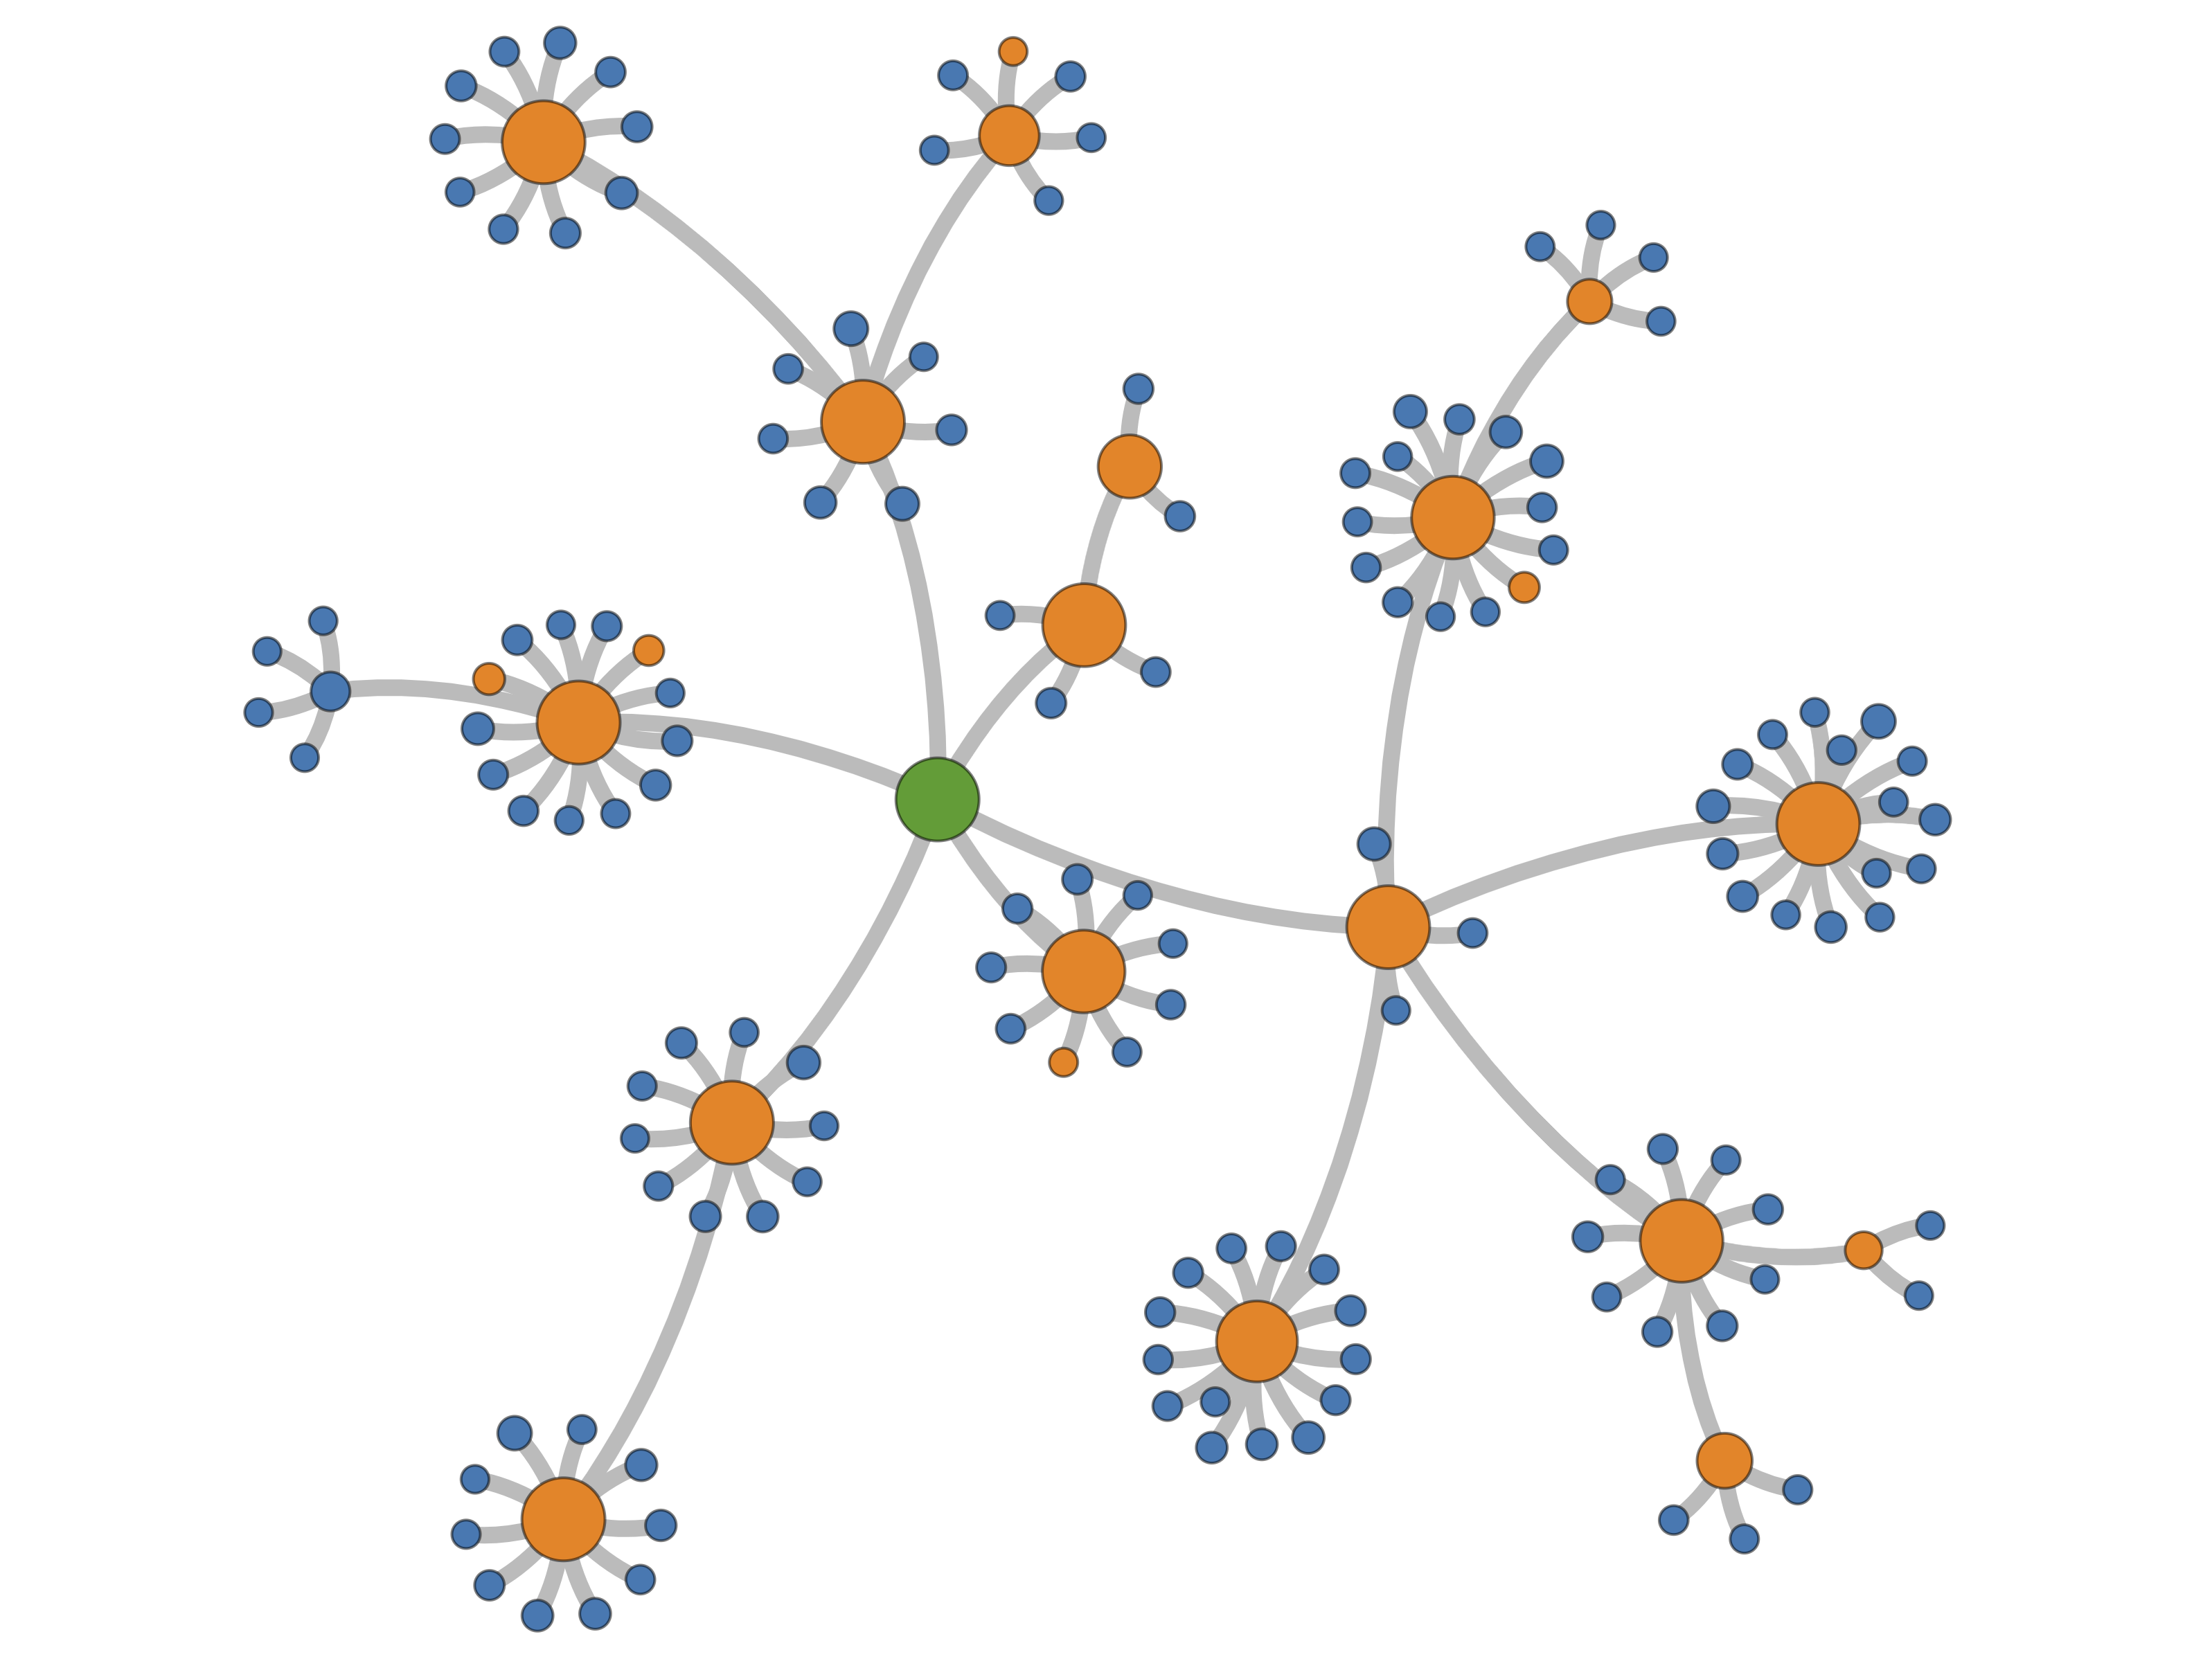
\includegraphics[width=\textwidth]{figures/synthetic 1}
\caption{Results.}
\label{fig:25-character model 1}
\end{figure}
%
\begin{figure}[htbp]
  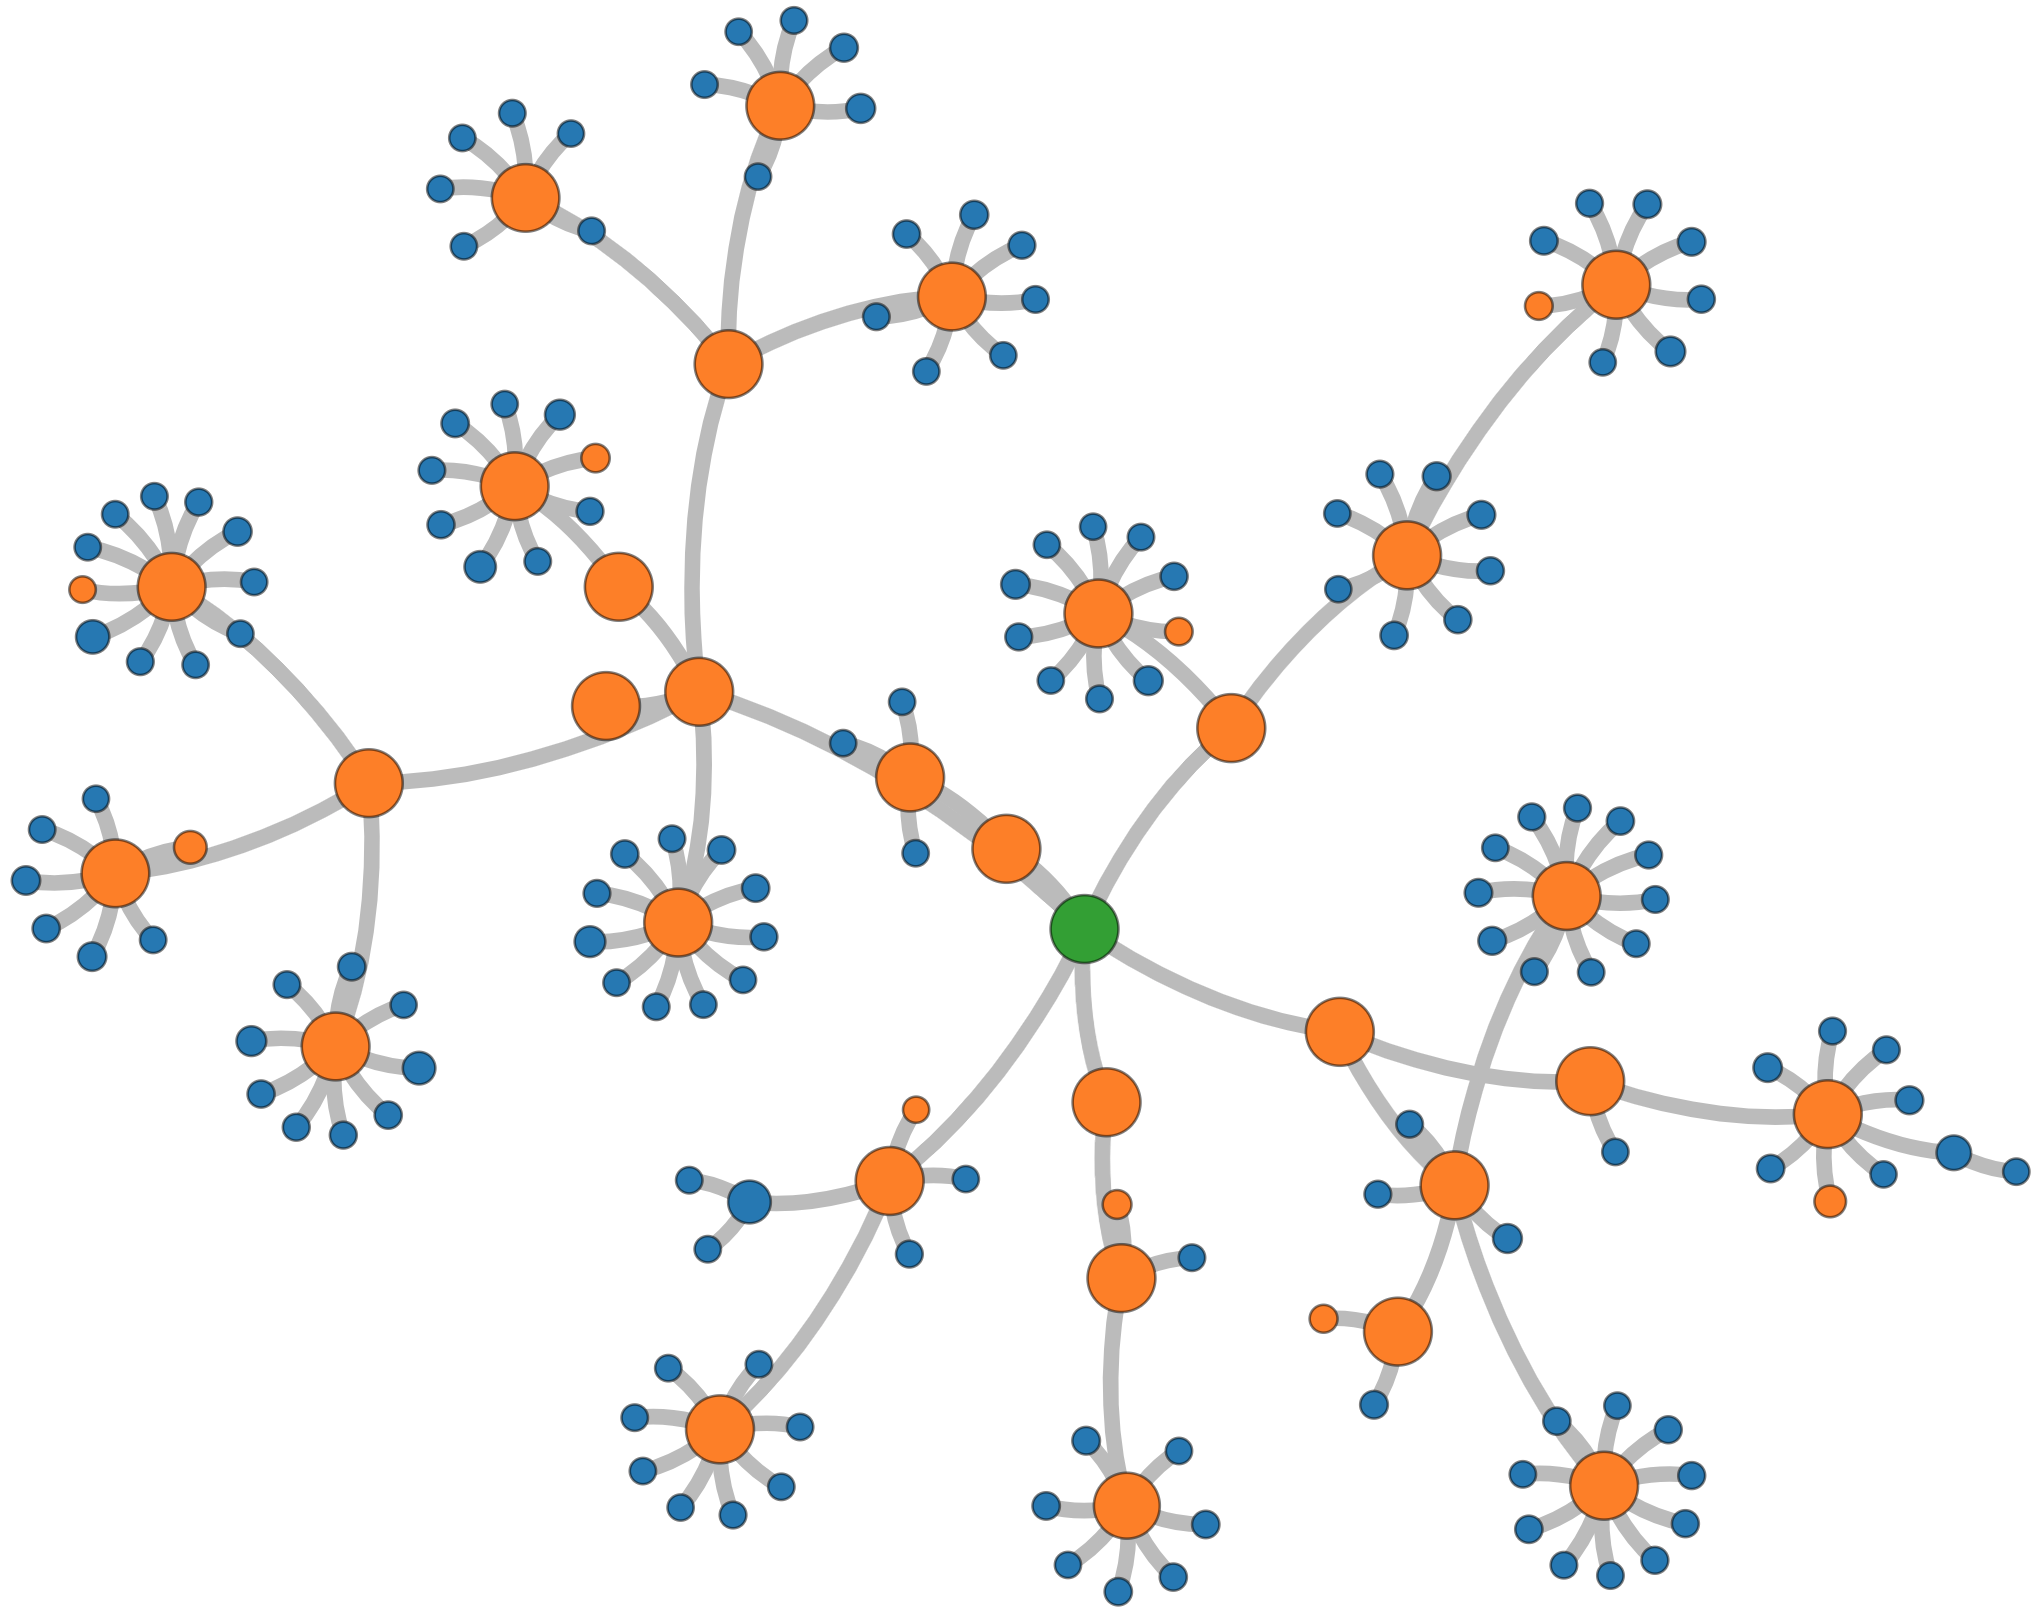
\includegraphics[width=\textwidth]{figures/synthetic 3}
\caption{Results.}
\label{fig:25-character model 2}
\end{figure}

\subsection{Text data}\label{sec:text} %========================================

In this and the next two sections we look for dependencies between symbols in
real-world data sets. To begin with, we consider two (English) text data sets:
the first is John Keats's \textit{Ode on Melancholy}, and the second
\textit{David Copperfield} by Charles Dickens.

Before any inference could be performed on the data sets, some preprocessing was
performed: characters were converted to lower case, punctuation marks other than
those that appear within words---such as apostrophes and hyphens---were removed,
and all whitespace characters were treated identically.

We consider two straightforward ways of viewing bodies of text as sequences: by
treating either characters or words as symbols. In the former case the symbol
alphabets for the two documents are of sizes~26 and~41 (for Keats and Dickens
respectively), and the lengths of the data sets are~1\,223 and~1\,843\,427. When
considering \emph{words} as symbols, the alphabets contain~157 and~15\,289
symbols respectively, and the sequences are of lengths~223 and~357\,043.

Inference results for the per-character case are summarised in tree form in
Figures~\ref{fig:text 1c} and~\ref{fig:text 2c}. Marginal probabilities were
estimated based on 100\,000 sampled models, and trees were constructed using
those states whose probabilities were greater than or equal to~0.1. Considering
the significant size difference between the two data sets (and thus support for
reoccurring subsequences), it is not surprising that the \textit{David
Copperfield} tree contains far more nodes than that of \textit{Ode on
Melancholy}.

Although a full description of the results is not possible here (at least not
for the Dickens book), we have gathered a few of the highest-probability states
from each simulation together in Tables~\ref{tab:text 1} and~\ref{tab:text 2}.
One sees, for example, that the prefix~`jo' is present in the Keats tree due to
its two occurrences as part of the word `joy'; or that in the Dickens work,~`mf'
is considered a significant prefix because it is almost followed by the
symbol~`o'---as in the word~`comfort' and its various derivatives.

Rather more specific, interesting prefixes arise in the Dickens text as well,
for example the five-character prefix~`the␣h', which also includes a whitespace
symbol. A number of related prefixes are present in the inferred state tree, all
with marginal probabilities greater than~0.9:~`␣h', `e␣h', `he_h', `the_h',
`f␣h', and~`u␣h'. Each of these states implies a slightly different distribution
over the vowel that follows the letter~`h'.

A histogram showing the overall distribution of the marginal probabilities
inferred from \textit{David Copperfield} is also given in Figure~\ref{fig:text
2c hist}---the fact that most of the probabilities are close to either~0 or~1 is
encouraging.

Treating documents as sequences of words is understandably far more challenging
than making use of individual characters, because doing so increases the size of
the symbol alphabet exponentially. In the case of the Keats poem these sizes
remain manageable, however the Dickens book could not be processed in full on
our MacBook Pro.\footnote{It is worth mentioning here that our implementation of
the inference algorithm was intended as a proof-of-concept, and although care
was taken to make the code efficient, it is by no means optimal. A more
efficient version would be written in a language other than Python and involve
fewer unnecessary memory allocations, but would also have taken significantly
longer to write.} Nonetheless, we have included the resulting state trees as
Figures~\ref{fig:text 1w} and~\ref{fig:text 2w}, and provided samples of the
inferred probabilities output in the two tables mentioned above as well.

Notice that only three of the words present in the Keats poem have estimated
probabilities greater than~0.5:~`and', `her', and~`the'. It is perhaps
interesting to see that these states have been assigned high probabilities even
though their empirical distributions are relatively flat (consisting of sets of
words that each only appear once); but these distributions are of course
significantly different to that of the root state~\(\lambda\), whose most likely
elements are~`the'~(14 occurrences), `of'~(8), `and`~(7), and~`her'~(6).
%
\begin{figure}[htbp]
\centering
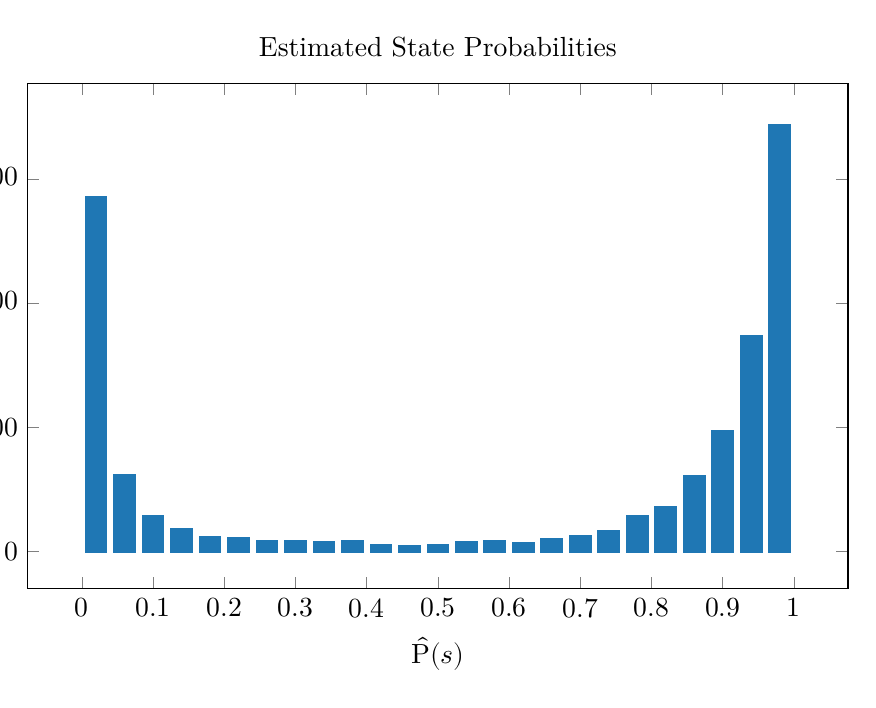
\begin{tikzpicture}[trim axis left, trim axis right]
\begin{axis}[
  title={Estimated State Probabilities},
  xlabel=\(\hat{\Pb}(s)\),
  ylabel={Frequency},
  bar width=7pt,
  width=12cm,
  height=8cm
]
  \addplot[ybar,cbblue,fill=cbblue]
    coordinates{(0.02, 1425) (0.06, 304) (0.1, 141) (0.14, 88) (0.18, 55)
      (0.22, 51) (0.26, 38) (0.3, 40) (0.34, 34) (0.38, 38) (0.42, 24)
      (0.46, 19) (0.5, 24) (0.54, 34) (0.58, 40) (0.62, 33) (0.66, 47) (0.7, 59)
      (0.74, 81) (0.78, 141) (0.82, 177) (0.86, 300) (0.9, 482) (0.94, 864)
      (0.98, 1715)};
\end{axis}
\end{tikzpicture}
\caption{Results.}
\label{fig:text 2c hist}
\end{figure}

\begin{table}[htbp]
\centering
\begin{tabular}{llccllc}
  \toprule
  \multicolumn{3}{c}{Characters} && \multicolumn{3}{c}{Words} \\
  \cmidrule{1-3} \cmidrule{5-7}
  \(s\) & \(\hat{\Pb}(s)\) & \(\argmax_x \ub{n}_s(x)\) &&
  \(s\) & \(\hat{\Pb}(s)\) & \(\argmax_x \ub{n}_s(x)\) \\
  \midrule
  a  & 1.0   & n: 18    && \(\lambda\) & 1.0   & the: 14                      \\
  c  & 0.308 & h: 5     && and         & 0.739 & be, let, \dots: 1            \\
  ee & 0.960 & p: 3     && her         & 0.870 & soft, rave, \dots: 1         \\
  ie & 0.106 & s: 4     && rich        & 0.102 & anger: 1                     \\
  an & 0.508 & d: 10    && soul        & 0.209 & but, shalt: 1                \\
  o  & 1.0   & r, u: 13 && that        & 0.206 & fosters, must: 1             \\
  jo & 0.426 & y: 2     && the         & 0.999 & beetle, death-moth, \dots: 1 \\
  t  & 0.916 & h: 28    && thy         & 0.368 & pale, sorrow, mistress: 1    \\
  \bottomrule
\end{tabular}
\caption{Example state probabilities derived from Keats's \textit{Ode on
  Melancholy}, when treated as a sequence of characters and words respectively.}
\label{tab:text 1}
\end{table}

\subsection{Temporal networks}\label{sec:temporal networks} %===================



\subsection{Genetic data}\label{sec:genetic} %==================================

\subsection{Unstructured data}\label{sec:unstructured} %========================

A simple, but nonetheless interesting test of our inference approach is to apply
it to unstructured data. In particular, we consider data generated according to
a single categorical distribution (i.e., using the trivial, single-state
model~\(\mc{S} = \{\lambda\}\)), and investigate the rate at which the marginal
probabilities of the non-trivial states converge to zero.

Recall that the state probabilities estimated by an MCMC simulation are always
non-decreasing along paths away from the root (e.g., \(\Pb(bc) \le \Pb(c) \le
\Pb(\lambda)\)), so we only need consider the probabilities assigned to the
root's direct children to obtain the maximum marginal probability over all
non-root states. We measure the rate at which this maximum decreases over data
sets that range in length from~10 to~10\,000 symbols, for three different
models.

The three models we consider have symbol alphabets of sizes~2, 10, and~20, and
as mentioned above, consits only of the root state~\(\lambda\). In the binary
case we consider two categorical distributions: the uniform distribution~\(\Pb(x
\peq 1) = 0.5\) as well as another chosen randomly. Since there is no
significant difference between the results for these two binary distributions,
we only consider uniform distributions when dealing with the 10- and
20-character models. Note that in the binary case, the model space was
restricted to that of \emph{full} binary trees, implying that the marginal
probabilities of the root's children were always equal: \(\hat{\Pb}(0) =
\hat{\Pb}(1)\).

Figure~\ref{fig:unstructured} shows the consolidated results for the three
models. For each model and each sequence length~\(\abs{\ub{x}}\), we
generated~20 random sequences according to the model's categorical distribution
and measured the maximum (non-root) marginal probability for each; the medians
and quartiles of these measurements were used to plot the traces in
Figure~\ref{fig:unstructured}. Each MCMC simulation was run until 10\,000
samples had been drawn.
%
\begin{figure}[htbp]
\centering
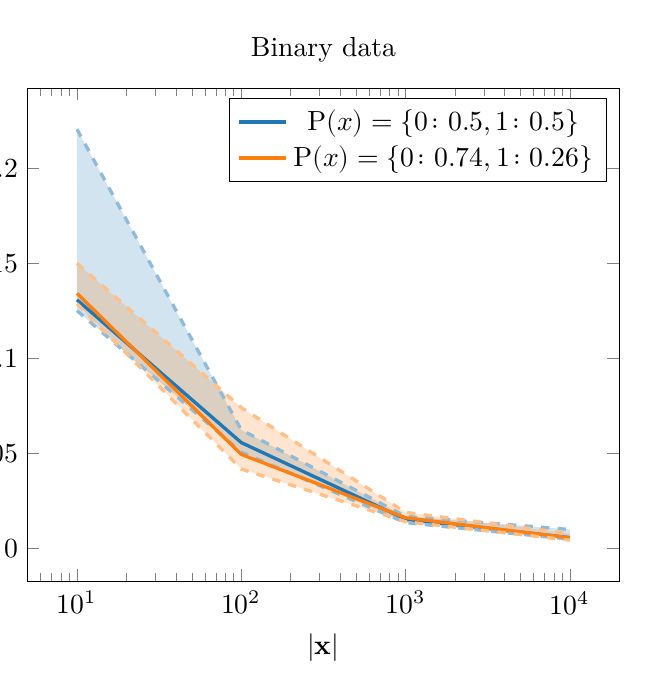
\begin{tikzpicture}[trim axis left, trim axis right]
\begin{semilogxaxis}[
  title={Binary data},
  xlabel=\(\abs{\ub{x}}\),
  ylabel=\(\ds \max_{s\ne\lambda} \Pb(s)\),
  yticklabel style={/pgf/number format/fixed},
  legend entries={
    {\(\Pb(x) = \{0\colon 0.5, 1\colon 0.5\}\)},
    {\(\Pb(x) = \{0\colon 0.74, 1\colon 0.26\}\)}
  }
]
  \addplot[cbblue,name path=median 1]
    coordinates{(10, 0.1308) (100, 0.0557) (1000, 0.0154) (10000, 0.0057)};
  \addplot[cbblue!50,dashed,name path=lower 1,forget plot]
    coordinates{(10, 0.1251) (100, 0.0507) (1000, 0.0136) (10000, 0.0049)};
  \addplot[cbblue!50,dashed,name path=upper 1,forget plot]
    coordinates{(10, 0.2205) (100, 0.0624) (1000, 0.0169) (10000, 0.01)};
  \addplot[cbblue,fill opacity=0.2,forget plot]
    fill between[of=lower 1 and upper 1];
  \addplot[cborange,name path=median 2]
    coordinates{(10, 0.1342) (100, 0.0495) (1000, 0.0162) (10000, 0.0056)};
  \addplot[cborange!50,dashed,name path=lower 2,forget plot]
    coordinates{(10, 0.1287) (100, 0.0418) (1000, 0.0141) (10000, 0.0044)};
  \addplot[cborange!50,dashed,name path=upper 2,forget plot]
    coordinates{(10, 0.15) (100, 0.0741) (1000, 0.019) (10000, 0.0078)};
  \addplot[cborange,fill opacity=0.2,forget plot]
    fill between[of=lower 2 and upper 2];
\end{semilogxaxis}
\end{tikzpicture}

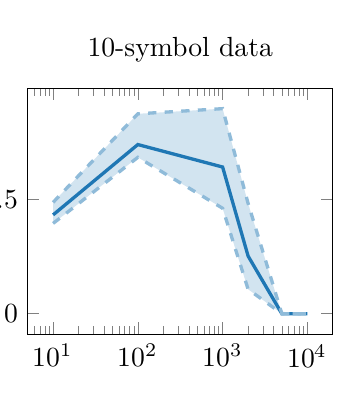
\begin{tikzpicture}[trim axis left, trim axis right]
\begin{semilogxaxis}[
  width=0.45\textwidth,
  title={10-symbol data},
  ytick={0,0.5,1}
]
  \addplot[cbblue,name path=median 1]
    coordinates{(10,   0.4333) (100,   0.7417) (1000, 0.6431) (2000, 0.2526)
                (5000, 0.0000) (10000, 0.0000)};
  \addplot[cbblue!50,dashed,name path=lower 1,forget plot]
    coordinates{(10,   0.3958) (100,   0.6856) (1000, 0.4623) (2000, 0.1070)
                (5000, 0.0000) (10000, 0.0000)};
  \addplot[cbblue!50,dashed,name path=upper 1,forget plot]
    coordinates{(10,   0.4882) (100,   0.8765) (1000, 0.8991) (2000, 0.4834)
                (5000, 0.0001) (10000, 0.0000)};
  \addplot[cbblue,fill opacity=0.2,forget plot]
    fill between[of=lower 1 and upper 1];
\end{semilogxaxis}
\end{tikzpicture}
\qquad
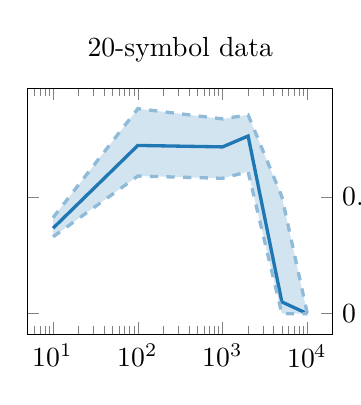
\begin{tikzpicture}[trim axis left, trim axis right]
\begin{semilogxaxis}[
  width=0.45\textwidth,
  title={20-symbol data},
  ytick={0,0.5,1},
  yticklabel pos=upper
]
  \addplot[cbblue,name path=median 1]
    coordinates{(10,   0.3658) (100,   0.7196) (1000, 0.7134) (2000, 0.7599)
                (5000, 0.0504) (10000, 0.0000)};
  \addplot[cbblue!50,dashed,name path=lower 1,forget plot]
    coordinates{(10,   0.3290) (100,   0.5887) (1000, 0.5791) (2000, 0.6074)
                (5000, 0.0000) (10000, 0.0000)};
  \addplot[cbblue!50,dashed,name path=upper 1,forget plot]
    coordinates{(10,   0.4108) (100,   0.8769) (1000, 0.8330) (2000, 0.8505)
                (5000, 0.5011) (10000, 0.0000)};
  \addplot[cbblue,fill opacity=0.2,forget plot]
    fill between[of=lower 1 and upper 1];
\end{semilogxaxis}
\end{tikzpicture}
\caption{Measurements of the maximum marginal probability of non-root model
  states for data sets of various sizes. Medians and quartiles derived from 20
  random sequences are shown for each model and each sequence
  length~\(\abs{\ub{x}}\).}
\label{fig:unstructured}
\end{figure}

The results depicted in Figure~\ref{fig:unstructured} are rather interesting:
although in the binary case the marginal probabilities of the non-trivial states
appear to decrease monotonically, and at a reasonable rate, the same cannot be
said of the 10- and 20-character models. For both of the larger models, the
maximum probability first \emph{increases} before finally decreasing, and the
values observed are often above~0.5, and occasionally near~1.

Although slightly unexpected, this behaviour is not difficult to explain: as the
number of symbols increases, the expected number of occurrences of each state in
a fixed-length sequence decreases. This implies that the empirical distributions
associated with these states---that is, the counts of the symbols that
immediately follow them in the sequence---are sparser. In addition, the chance
of at least one state having a markedly non-uniform distribution increases
naturally with the number of symbols. One also needs to take into account the
behaviour of each state's children (and their children, and so on), because the
empirical distributions associated with these states will influence the
estimated probabilities of their parents. Finally, the fact that the maximum
inferred probability appears to \emph{increase} at first is simply due to the
size of the first one or two data sets: they are too small for any non-uniform
behaviour to be of any real significance.

In the end it is a combination of the reasons given above that causes inference
on models with large symbol alphabets to converge relatively slowly (in terms of
data-set size). That being said, the traces shown in
Figure~\ref{fig:unstructured} tell a somewhat one-sided story: if one plots the
\emph{mean} marginal probability of the root's child nodes instead of the
maximum, one finds that in both the 10- and 20-character case, across all of the
tested sequence lengths, this mean never rises above~0.4. In both cases the
plots are monotonically decreasing from~\(\abs{\ub{x}} = 100\) onwards. Plots of
the median probability behave similarly.

\subsubsection{Asymptotic rate of convergence}\label{sec:asymptotic} %==========

To end this section, we give a quick derivation of the asymptotic rate at which
the marginal likelihood decreases with each attachment operation of a full
binary tree, as a function of the sequence length~\(n = \abs{\ub{x}}\). The idea
here is to quantify, for large \(n\), the effect that adding all of a leaf
node's children to the model has on the marginal likelihood~\(\Pb(\ub{x} \mid
\mc{S})\).

Recall from~\eqref{eqn:bayes factor} that if \(\mc{S}'\) is the model created by
attaching a node to a leaf~\(r\) of the state tree~\(\mc{S}\), then the ratio of
the two models' marginal likelihoods is:
\begin{equation}
  \frac{\Pb\lr{\ub{x} \mid \mc{S}'}}{\Pb\lr{\ub{x} \mid \mc{S}}} =
    \frac{\Beta\lr{\ub{n}_r + \ub{\alpha} \mid \mc{S}'}}
    {\Beta\lr{\ub{n}_r + \ub{\alpha} \mid \mc{S}}}
    \frac{\Beta\lr{\ub{n}_{0r} + \ub{\alpha}}}{\Beta\lr{\ub{\alpha}}}.
\end{equation}
Here we have assumed that the newly attached node represents the symbol~0, and
have labelled it as state \(0r\) accordingly. A full binary attachment involves
the attachment of a node representing the symbol~1 as well, and the ratio
involving the resulting model~\(\mc{S}''\) is:
\begin{equation}\label{eqn:bayes factor binary}
  \frac{\Pb\lr{\ub{x} \mid \mc{S}''}}{\Pb\lr{\ub{x} \mid \mc{S}}} =
    \frac{\Beta\lr{\ub{n}_r + \ub{\alpha} \mid \mc{S}''}}
    {\Beta\lr{\ub{n}_r + \ub{\alpha} \mid \mc{S}}}
    \frac{\Beta\lr{\ub{n}_{0r} + \ub{\alpha}}\,
    \Beta\lr{\ub{n}_{1r} + \ub{\alpha}}}{\Beta\lr{\ub{\alpha}}^2}.
\end{equation}

If the data set in question is simply a sequence of characters generated
according to the unstructured, uniform distribution~\(\Pb(x \peq 1) = 0.5\),
then for large enough~\(n\) the occurrence counts associated with any given
state will be roughly equal; that is, \(\ub{n}_s(0) \approx \ub{n}_s(1)\).
(Technically we can assume that~\(\ub{n}_s(1) - \ub{n}_s(0) = o(n)\), although
we omit this from the derivation below for the sake of brevity.) In particular,
the counts corresponding to the root state will satisfy~\(\ub{n}_{\lambda}
\approx (n/2, n/2)\) (recall that the root state represents the empty prefix,
which `occurs' before every character in the sequence); those associated with
the root's child~0 will be~\(\ub{n}_0 \approx (n/4, n/4)\); and so on.

Let~\(r = \lambda\) in the above equations, so that \(\mc{S}\) and \(\mc{S}''\)
are now the complete binary state trees of sizes~1 and~3 respectively. Note also
that when both children of the root are present (in~\(\mc{S}''\)), the
state~\(\lambda\) will only have an effective count of~1, which we without loss
of generality assume corresponds to the symbol~0. Using idealised---but
asymptotically valid---counts, we have:
\begin{align}\label{eqn:bayes factor asymptotic}
  \frac{\Pb(\ub{x} \mid \mc{S}'')}{\Pb(\ub{x} \mid \mc{S})} &=
    \frac{\Beta(\ub{n}_{\lambda} + \ub{\alpha} \mid \mc{S}'')}
    {\Beta(\ub{n}_{\lambda} + \ub{\alpha} \mid \mc{S})}
    \frac{\Beta(\ub{n}_0 + \ub{\alpha})\, \Beta(\ub{n}_1 + \ub{\alpha})}
    {\Beta(\ub{\alpha})^2} \nonumber \\
  &\sim \frac{\Beta\lr*{\lr*{1, 0} + \ub{\alpha}}\,
    \Beta\lr*{\lr*{\frac{n}{4}, \frac{n}{4}} + \ub{\alpha}}\,
    \Beta\lr*{\lr*{\frac{n}{4}, \frac{n}{4}-1} + \ub{\alpha}}}
    {\Beta\lr*{\lr*{\frac{n}{2}, \frac{n}{2}} + \ub{\alpha}}\,
    \Beta(\ub{\alpha})^2}.
\end{align}

We can treat this equation in parts, starting with the constant terms. To
simplify the derivation we also assume that the concentration parameter is
symmetric:~\(\ub{\alpha} = (\alpha, \alpha, \dots)\).
\begin{align*}
  \frac{\Beta((1, 0) + \ub{\alpha})}{\Beta(\ub{\alpha})^2} &=
    \frac{\Gamma(1 + \alpha)\, \Gamma(\alpha)}{\Gamma(1 + 2\alpha)}
    \frac{\Gamma(2\alpha)}{\Gamma(\alpha)\, \Gamma(\alpha)}
    \frac{1}{\Beta(\ub{\alpha})} \\
  &= \frac{1}{2\Beta(\ub{\alpha})}.
\end{align*}

The terms that are dependent on~\(n\) can be simplified using Stirling's
formula, e.g.:
\begin{align*}
  \Beta\lr*{\lr*{\frac{n}{4}, \frac{n}{4}} + \ub{\alpha}} &\sim
    \sqrt{2\pi}\, \frac{\lr*{\frac{n}{4} + \alpha}^{(n/4)+\alpha-(1/2)}
    \lr*{\frac{n}{4} + \alpha}^{(n/4)+\alpha-(1/2)}}
    {\lr*{\frac{n}{2} + 2\alpha}^{(n/2)+2\alpha-(1/2)}} \\
  &\sim \sqrt{2\pi}\, \frac{\lr*{\frac{n}{4}}^{(n/4)+\alpha-(1/2)}
    \lr*{\frac{n}{4}}^{(n/4)+\alpha-(1/2)}}
    {\lr*{\frac{n}{2}}^{(n/2)+2\alpha-(1/2)}}.
\end{align*}
Applying this to the three dependent terms yields:
\begin{align*}
  \frac{\Beta\lr*{\lr*{\frac{n}{4}, \frac{n}{4}} + \ub{\alpha}}\,
    \Beta\lr*{\lr*{\frac{n}{4}, \frac{n}{4}-1} + \ub{\alpha}}}
    {\Beta\lr*{\lr*{\frac{n}{2}, \frac{n}{2}} + \ub{\alpha}}}
  &\sim \sqrt{2\pi}\, \frac{\lr*{\frac{n}{4}}^{3((n/4)+\alpha-(1/2))}
    \lr*{\frac{n}{4}}^{(n/4)+\alpha-(3/2)}}
    {\lr*{\frac{n}{2}}^{(n/2)+2\alpha-(1/2)}
    \lr*{\frac{n}{2}}^{(n/2)+2\alpha-(3/2)}} \\
  &\times \frac{n^{n+2\alpha-(1/2)}}
    {\lr*{\frac{n}{2}}^{2((n/2)+\alpha-(1/2))}} \\
  &= \sqrt{2\pi}\, \frac{\lr*{\frac{n}{4}}^{n+4\alpha-3} n^{n+2\alpha-(1/2)}}
    {\lr*{\frac{n}{2}}^{2n+6\alpha-3}} \\
  &= \sqrt{2\pi}\, 2^{3-2\alpha} n^{-1/2}.
\end{align*}

Putting the constant and dependent terms together, Equation~\eqref{eqn:bayes
factor asymptotic} reduces to:
\begin{equation}\label{eqn:bayes factor asymptotic 2}
  \frac{\Pb(\ub{x} \mid \mc{S}'')}{\Pb(\ub{x} \mid \mc{S})} \sim
    \frac{\sqrt{2\pi}}{\Beta(\ub{\alpha})} 4^{1-\alpha} n^{-1/2}.
\end{equation}
What this means is that in the case of uniformly random binary data, the
marginal likelihood of a three-node, complete state tree is smaller than that of
the single-node model by a factor that is~\(\Theta(n^{-1/2})\) for large~\(n =
\abs{\ub{x}}\). The same goes for larger state trees: attaching a pair of nodes
to a leaf of the three-node tree to form a five-node model will further reduce
the marginal likelihood by a factor of order~\((n/2)^{-1/2}\) (because roughly
half of the characters in the sequence match the existing state), and so on.

Of course we have not been dealing with the marginal likelihoods of individual
models up until now; rather, we have been interested in \emph{sums} of marginal
likelihoods over models that include a particular node~\(s\). With a bit of work
though, we can extend the asymptotic expression derived above to such sums as
well.

\section{Implementation notes} %================================================

\end{document}